\documentclass[aspectratio=169]{beamer}

\usetheme{Madrid}
\usecolortheme{seahorse}
\setbeamertemplate{navigation symbols}{}
\setbeamertemplate{footline}[frame number]

\usepackage{amsmath,amssymb}
\usepackage{booktabs}
\usepackage{graphicx}
\usepackage{xcolor}

\graphicspath{{paper_assets/}}

\newcommand{\E}{\mathbb{E}}
\newcommand{\Var}{\operatorname{Var}}
\newcommand{\norm}[1]{\left\lVert #1 \right\rVert}
\newcommand{\CV}{\operatorname{CV}}
\newcommand{\btheta}{\boldsymbol{\theta}}
\newcommand{\bbeta}{\boldsymbol{\beta}}

% XXX FIX THIS
\title{Are you stressed? Bayesian Regime Detection in Crypto Markets}
\subtitle{Learning Which Data Matters for Scalable HMM Inference}
\author{Diego Luca Gonzalez Gauss, Enrico Yao-Bate, Haozhe Yang}
\institute{STAT 221 Spring 2026 Final Project}
\date{May 5, 2026}

\begin{document}

\begin{frame}
  \titlepage
\end{frame}

\begin{frame}{The high-level question}
  \Large
  Can we do scalable Bayesian regime inference for crypto returns?

  \vspace{0.8em}
  \normalsize
  \begin{block}{Why this is interesting}
    Crypto markets switch between calm, stress, and chaos regimes. If we can infer which regime we are in, fast and with calibrated uncertainty, we get risk control and drawdown avoidance.
  \end{block}

  \begin{block}{Why this is hard}
    The natural model for regime-switching is a Hidden Markov Model (HMM). But HMM posteriors are expensive to compute, and the standard tools for scaling inference introduce new problems of their own.
  \end{block}
\end{frame}

\begin{frame}{Why an HMM for crypto returns?}
  \begin{columns}[T]
    \begin{column}{0.55\linewidth}
      Crypto assets go through extended periods of low volatility where daily returns are small and centered near zero. Then, abruptly, daily moves of 10-20\% become common, correlations spike, and drawdowns cascade across assets. These shifts are discrete, not gradual. An HMM captures this:
      \begin{itemize}
        \item Latent state $z_t \in \{1, \dots, K\}$: market regime.
        \item Return distribution depends on the regime:
        \[
          y_t \mid z_t=k \sim \mathcal{N}(\mu_k, \Sigma_k).
        \]
        \item Regimes tend to persist, i.e. if we are in calm today, we are likely in calm tomorrow:
        \[
          z_t \mid z_{t-1} \sim \operatorname{Categorical}(A_{z_{t-1},:}).
        \]
      \end{itemize}
    \end{column}
    \begin{column}{0.40\linewidth}
      \begin{block}{Example states}
        0: calm / low volatility.

        1: stressed / increasing volatility.

        2: chaos / extreme volatility
      \end{block}
    \end{column}
  \end{columns}
\end{frame}

\begin{frame}{Why MCMC?}
  We want the full posterior $p(z_t \mid y_{1:T}, \btheta)$ over model parameters and latent states. But it is complex because it is high-dimensional (transition matrix, emission parameters for each state) and involves discrete latent variables.

  \vspace{0.5em}
  \begin{itemize}
    \item EM gives a point estimate but no uncertainty quantification.
    \item Variational methods require choosing an approximating family, which can miss important posterior structure.
    \item MCMC targets the exact posterior.
  \end{itemize}

  \vspace{0.3em}
  \begin{block}{The problem}
    MCMC requires the full posterior gradient at every step. For an HMM, this means an $O(TK^2)$ forward-backward pass over the entire series. For long series, this is prohibitive.
  \end{block}
\end{frame}

\begin{frame}{Why stochastic-gradient MCMC?}
  The idea is that because the HMM log-posterior decomposes as a sum over time, instead of computing the full gradient, we can approximate it by sampling $M$ block indices $I_1, \dots, I_M$ from a distribution $p$ over the $B$ blocks, and reweighting by their sampling probabilities:
  \[
    \widehat G(\btheta)=
    \nabla\log p(\btheta)
    +
    \frac{1}{M}\sum_{m=1}^M
    \frac{g_{I_m}(\btheta)}{p_{I_m}},
    \qquad g_b(\btheta)=\nabla \ell_b(\btheta).
  \]

  SGLD update (Welling \& Teh, 2011):
  \[
    \btheta_{t+1} = \btheta_t + \frac{\eta_t}{2}\,\widehat{G}(\btheta_t) + \xi_t, \qquad \xi_t \sim \mathcal{N}(0, \eta_t\, I).
  \]
\end{frame}

\begin{frame}{The lower-level question}
  \Large
  How should we set the block sampling distribution $p$?

  \vspace{0.8em}
  \normalsize
  A first-pass answer is uniform sampling $p_b = 1/B$ since it is unbiased and simple. However, it ignores the fact that not all blocks are equally informative. 
  
  \vspace{0.5em}
  In crypto, most blocks capture sideways price action, and only a few contain crashes, liquidation cascades, or regime transitions. These rare blocks carry most of the gradient signal for stress-regime parameters, meaning that if we consistently under-sample them, we may lose the ability to accurately detect when the market is entering or exiting a stress regime.

  \vspace{0.5em}
  \begin{block}{The statistical computing question}
    How should we set the block sampling distribution $p$ in SG-MCMC for HMMs to ensure rare but informative regimes are adequately represented in the gradient estimate?
  \end{block}
\end{frame}

\begin{frame}{An existing answer: TASS (Ou, Young, Sen, Dunson, 2024)}
  \begin{block}{Their answer}
    Sample each block in proportion to how much gradient signal it carries, so blocks that matter more for the posterior get sampled more often.
  \end{block}

  \vspace{0.3em}
  Formally, we want to choose sampling weights $a_n$ that minimize the variance of our stochastic gradient estimator $\E\|\widehat{\nabla} - \nabla\|^2$. If we knew the latent states $z_t$, we could compute each block's gradient contribution
  \[
    g_n(\btheta) = \sum_{t \in C_n} \nabla_{\btheta} \left[\log p(y_t \mid z_t) + \log p(z_t \mid z_{t-1})\right].
  \]
  and just as we set proposal weights proportional to the integrand in importance sampling, the variance-optimal thing to do here is to set block weights $a_n^\star$ proportional to gradient norms.

  \vspace{0.3em}
  \textbf{Problem:} these weights require knowing the latent states $z_t$, which are exactly what we are trying to infer, and the current parameter $\btheta$, which changes at every MCMC step.
\end{frame}

\begin{frame}{How TASS approximates optimal weights in practice}
  \begin{enumerate}
    \item \textbf{Cluster observations:} run $K$-means on $y_1, \ldots, y_T$ to get proxy state labels $\hat{z}_t$. 
    \item \textbf{Compute approximate block gradients:} evaluate the block gradient formula with $\hat{z}_t$ in place of $z_t$ and $\btheta$ fixed at $\btheta_{\mathrm{MAP}}$:
      \[
        \tilde{g}_n = \sum_{t \in C_n} \nabla_{\btheta} \left[\log p(y_t \mid \hat{z}_t) + \log p(\hat{z}_t \mid \hat{z}_{t-1})\right]\bigg|_{\btheta = \btheta_{\mathrm{MAP}}}.
      \]
    \item \textbf{Set weights:}
      $\displaystyle\tilde{a}_n = \frac{\norm{\tilde{g}_n}}{\sum_{n'=1}^{N}\norm{\tilde{g}_{n'}}}$ so blocks with many rare-state observations get large $\tilde{a}_n$.
    \item \textbf{Sample:} draw blocks with probabilities
      $\displaystyle p_n^{\mathrm{TASS}} = (1-\lambda)\,\tilde{a}_n + \frac{\lambda}{N},$ where the $\lambda/N$ is to ensure every block still has a chance to be sampled.
  \end{enumerate} 

  \vspace{0.3em}
  \begin{block}{Limitation}
    TASS weights are static. They only use emission values (through $K$-means), and cannot adapt if the importance of blocks shifts as the chain explores the posterior.
  \end{block}
\end{frame}

\begin{frame}{Our answer: learn which blocks matter during sampling}
    \begin{block}{High-level idea}
      Replace the static weights with a model that predicts each block's gradient importance from observable features, and updates those predictions during sampling using gradient feedback.
    \end{block}

  \vspace{0.5em}
  For each block $C_n$, we compute a feature vector $w_n \in \mathbb{R}^p$ from the observations in that block:
  \begin{itemize}
    \item mean absolute return, mean squared return,
    \item rolling volatility (within-block standard deviation),
    \item cross-sectional dispersion (spread across similar assets),
    \item tail event counts (number of returns exceeding a threshold),
    \item downside pressure (fraction of negative returns).
  \end{itemize}
  These are observable proxies for regime activity since stress blocks tend to have high volatility, large returns, and high dispersion.
\end{frame}

\begin{frame}{The online weight model}
  Recall from TASS that the optimal weight for block $n$ is $a_n^\star \propto \|g_n(\btheta)\|$. We want to predict this from the block features $w_n$, and update the prediction as $\btheta$ changes during sampling. 

  \vspace{0.5em}
  We opt to do this by turning it into a regression problem. Gradient norms are positive and vary over orders of magnitude, so we model the log-squared norm as linear in features:
  \[
    \log \norm{g_n(\btheta_t)}^2 \;\approx\; \widehat\bbeta_t^\top w_n,
  \]
  where $\widehat\bbeta_t \in \mathbb{R}^p$ is a coefficient vector, updated at each MCMC step $t$, that captures how each feature relates to gradient importance. This gives natural importance weight estimates
  \[
    \widehat a_{n,t} = \exp\!\bigl(\tfrac{1}{2}\,\widehat\bbeta_t^\top w_n\bigr) \;\approx\; \norm{g_n(\btheta_t)}.
  \]

  \vspace{0.5em}
  As in TASS, we convert weights to sampling probabilities with a uniform exploration floor:
  \[
    p_{n,t}
    =
    (1-\lambda)\,
    \frac{\widehat a_{n,t}}{\sum_{n'=1}^N \widehat a_{n',t}}
    +
    \frac{\lambda}{N}.
  \]
\end{frame}

\begin{frame}{Fitting $\widehat\bbeta_t$ by discounted ridge regression}
  At each SGLD step $t$, after sampling block $C_{n_s}$ and computing its gradient, we observe what we call the \textbf{feedback response} for our regression:
  \[
    f_s = \log\bigl(\norm{g_{n_s}(\btheta_s)}^2 + \epsilon\bigr),
  \]
  where $\epsilon > 0$ prevents $\log 0$. We now have a training pair $(w_{n_s},\, f_s)$ and can update $\widehat\bbeta_t$.

  \vspace{0.3em}
  We need a regression method that (a) adapts to non-stationarity, since block importance shifts as $\btheta$ moves, and (b) has a cheap closed-form update, since it runs inside every SGLD step. Discounted ridge regression satisfies both, so we do
  \[
    \widehat\bbeta_t
    =
    \arg\min_{\bbeta}
    \sum_{s < t}
    \rho^{t-s}
    \bigl(f_s - \bbeta^\top w_{n_s}\bigr)^2
    +\tau\norm{\bbeta}^2,
  \]
  where the \textbf{discount} $\rho \in (0,1)$  down-weights old observations exponentially, so the model tracks shifting importance rather than averaging over the entire chain history, while our \textbf{ridge penalty} $\tau > 0$ regularizes early in the chain when few blocks have been sampled.

  \vspace{0.5em}
  This has a closed-form recursive update ($O(p^2)$ per step), so it is cheap enough to run inside every SGLD iteration
\end{frame}

\begin{frame}{When does online beat static?}
  Write $a_n = \norm{g_n(\btheta)}$ for the true gradient norm of block $n$. The stochastic gradient variance under uniform sampling is inflated by a factor of
  \[
    1 + \CV(a)^2,
    \qquad
    \text{where } \CV(a) = \frac{\mathrm{sd}(a_1,\ldots,a_N)}{\mathrm{mean}(a_1,\ldots,a_N)}.
  \]
  When gradient norms are heterogeneous across blocks (high $\CV$), uniform sampling wastes most of its budget on low-signal blocks.

  \vspace{0.3em}
  Online beats uniform whenever its prediction error $\varepsilon$ (worst-case log-ratio between predicted and true weights) satisfies
  \[
    \frac{e^{2\varepsilon}}{1-\lambda}
    <
    1+\CV(a)^2.
  \]

  \begin{center}
    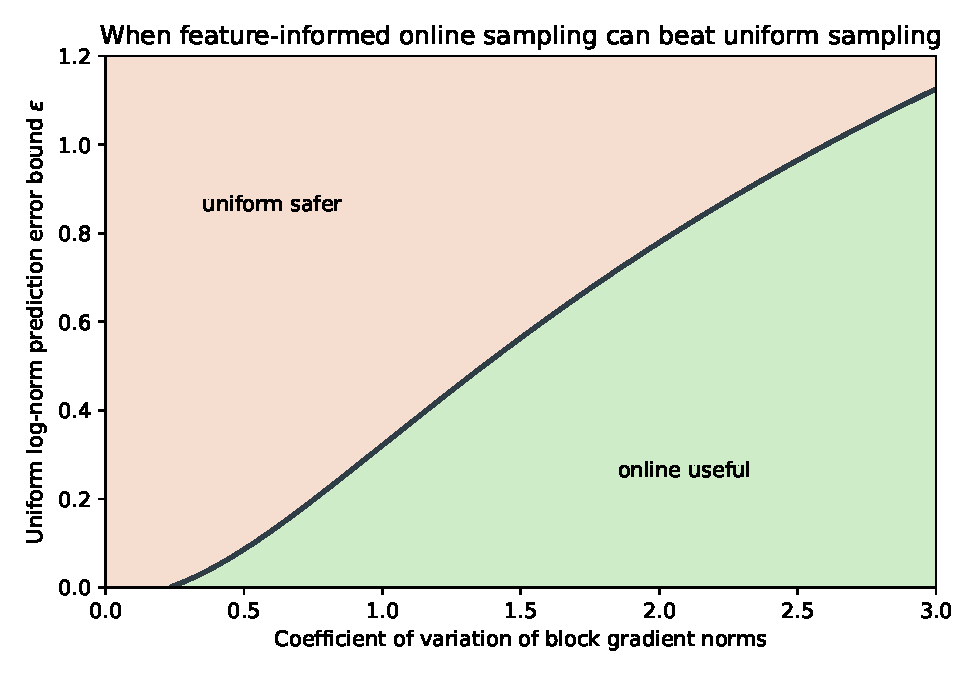
\includegraphics[height=0.35\textheight]{online_usefulness_region.pdf}
  \end{center}
  \small In crypto with rare stress regimes, $\CV$ is large and our features predict well $\Rightarrow$ online weighting helps.
\end{frame}

\begin{frame}{Scale down to an actual crypto task}
  \begin{block}{Forward-looking target}
    At the end of each 10-day block, predict whether the next 10-day equal-weight crypto basket return is a stress event:
    \[
      y_b=\mathbf 1\{R_{b+1}^{\mathrm{mkt}}\le -7\%\}.
    \]
  \end{block}

  \begin{block}{Features}
    Current-block return, volatility, drawdown, downside pressure, cross-asset dispersion, tail counts, and asset-specific vol/downside summaries.
  \end{block}

  \begin{alertblock}{This is a real crypto question}
    Should we be risk-on or risk-off for the next two weeks?
  \end{alertblock}
\end{frame}

\begin{frame}{Why this task is covered by the math}
  Fit a logistic stress model:
  \[
    h_\beta(w_b)=\sigma(\beta^\top w_b),
    \qquad
    \ell_b(\beta)=\text{cross-entropy}(y_b,h_\beta(w_b)).
  \]

  The block gradient is
  \[
    g_b(\beta)=\nabla \ell_b(\beta)
    =
    \{h_\beta(w_b)-y_b\}w_b.
  \]

  \begin{block}{Same useful-regime condition}
    If a few blocks are high-loss/high-gradient, and cheap crypto features predict them, online weighting should improve stochastic training.
  \end{block}

  \begin{block}{Why static can get stale}
    The stress signature changes: volatility, downside skew, dispersion, liquidation-like tails. Online can track; frozen weights cannot.
  \end{block}
\end{frame}

\begin{frame}{Actual crypto task results}
  \centering
  \resizebox{0.94\linewidth}{!}{\begin{tabular}{lrrrrrr}
\toprule
Method & Log loss & Brier & AUC & Top-risk stress rate & Strategy return & Max drawdown \\
\midrule
Online & 0.524 & 0.172 & 0.625 & 37.5\% & -33.3\% & -49.5\% \\
Static TASS & 0.531 & 0.175 & 0.623 & 25.0\% & -25.0\% & -48.3\% \\
Uniform & 0.533 & 0.176 & 0.620 & 25.0\% & -41.5\% & -55.1\% \\
Buy-and-hold & -- & -- & -- & -- & -49.7\% & -65.1\% \\
\bottomrule
\end{tabular}
}

  \vspace{0.7em}
  \begin{block}{Readout}
    Online has the best log loss, Brier score, AUC, and top-risk stress concentration.
  \end{block}

  \begin{alertblock}{Trading caveat}
    Static TASS wins this simple total-return threshold rule. Online is the cleanest risk forecaster; trading P\&L is a noisy downstream functional.
  \end{alertblock}
\end{frame}

\begin{frame}{Online risk scores over time}
  \begin{center}
    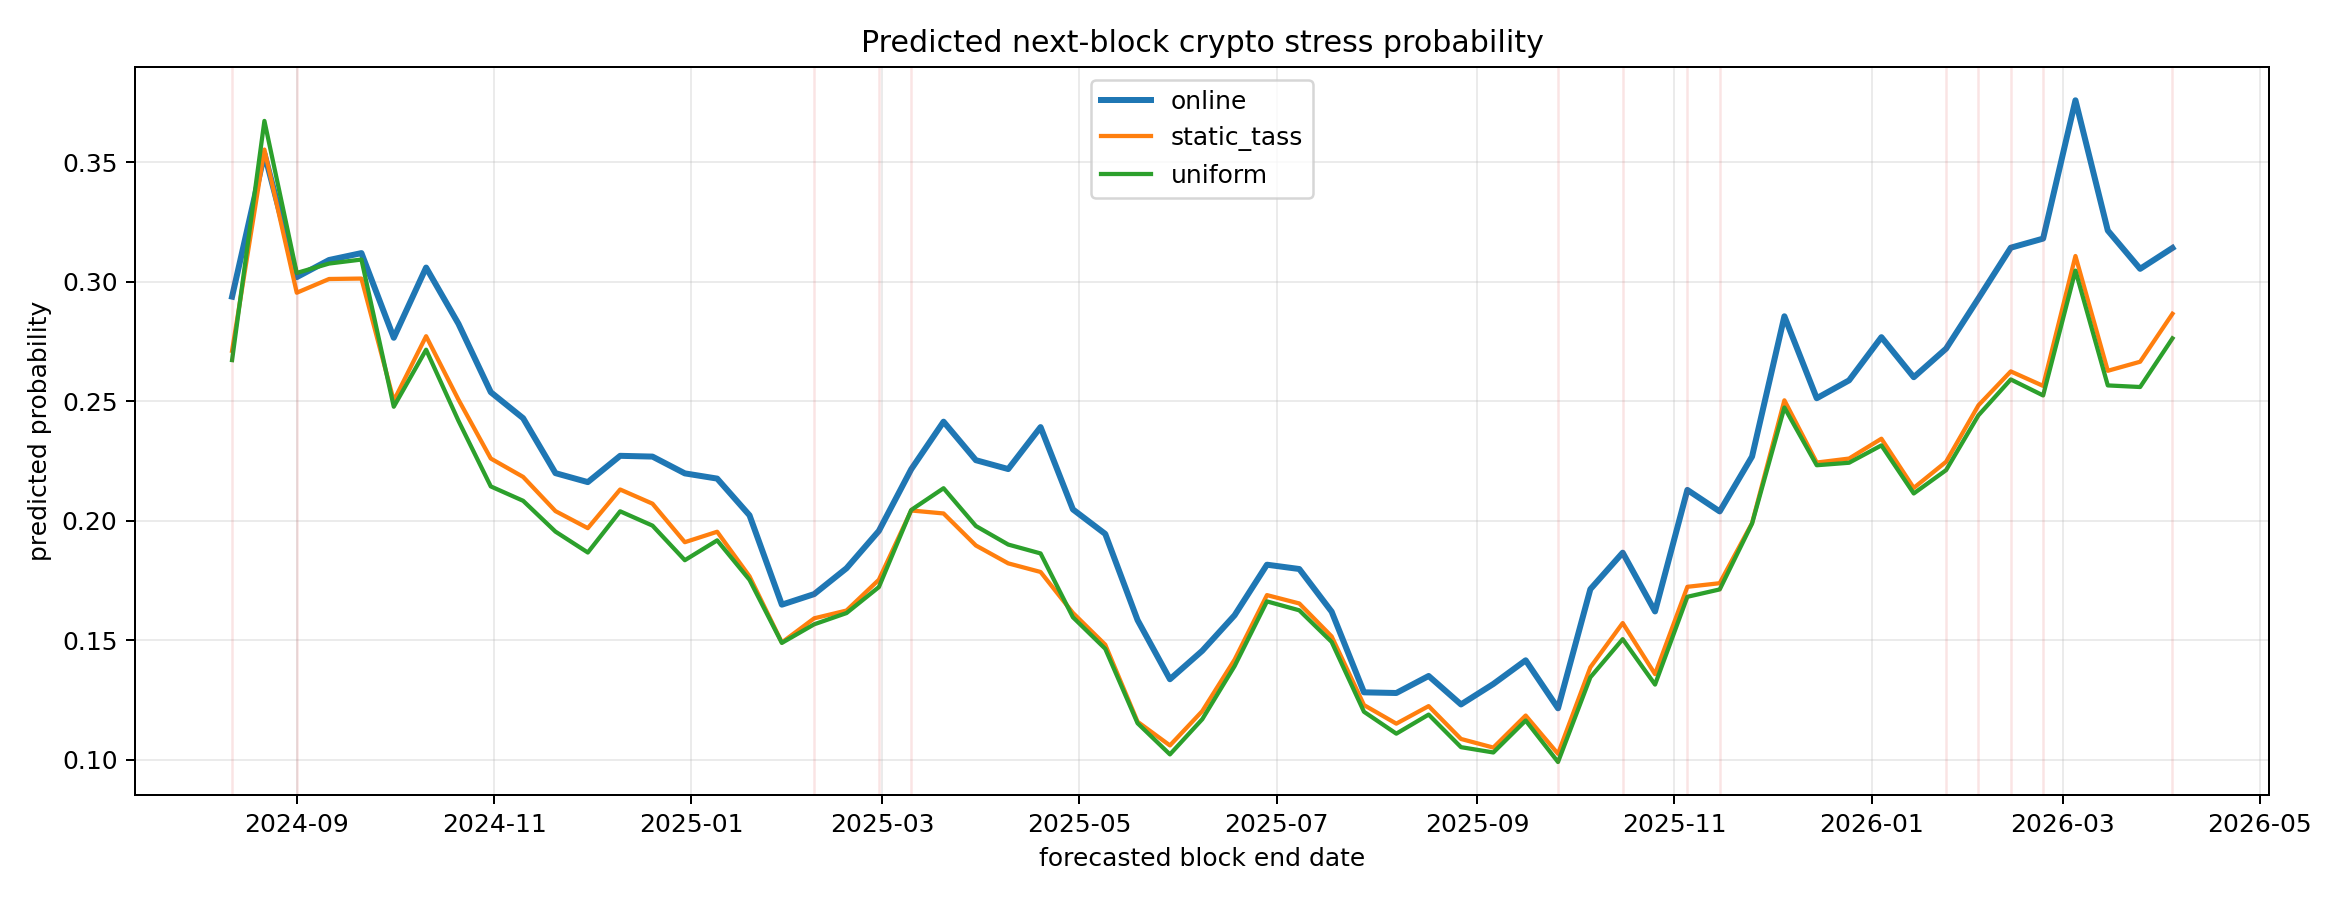
\includegraphics[width=0.92\linewidth]{actual_crypto_predicted_stress_probability.png}
  \end{center}
\end{frame}

\begin{frame}{Money-flavored diagnostic}
  \begin{center}
    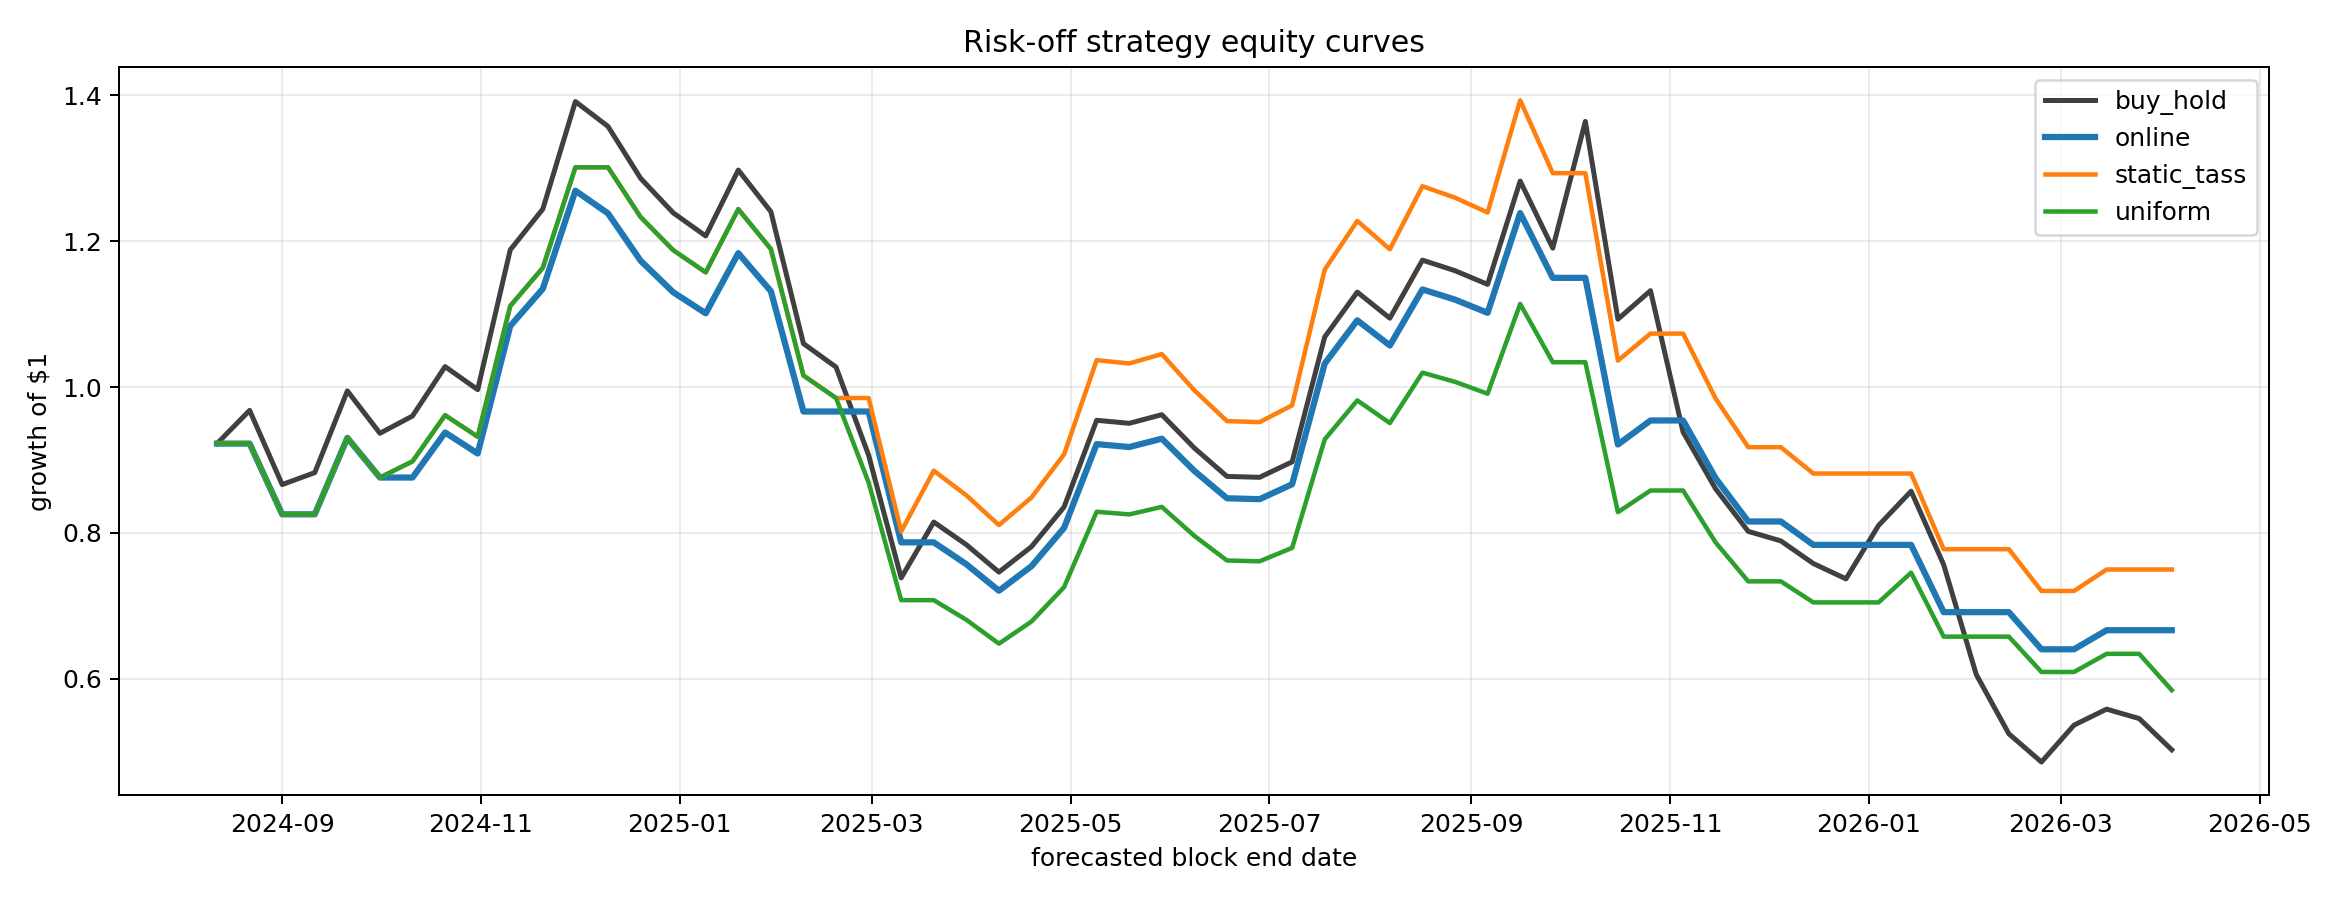
\includegraphics[height=0.58\textheight]{actual_crypto_risk_off_equity_curves.png}
  \end{center}

  \begin{block}{Interpretation}
    \small
    The risk-off rule is intentionally simple: hold crypto unless predicted stress is top-quartile, then hold cash.
  \end{block}
\end{frame}

\begin{frame}{Then we tried to scale to full HMM inference}
  \begin{block}{The hope}
    Use the same targeted weighting idea inside SGLD for Bayesian HMM posterior sampling.
  \end{block}

  \begin{block}{The reality}
    Once the target is a full HMM posterior, gradient variance is no longer the only bottleneck.
  \end{block}

  \begin{itemize}
    \item Label switching and multimodality.
    \item Weakly identified third regime.
    \item Transition/covariance coupling.
    \item Finite-step SGLD bias and numerical stability constraints.
  \end{itemize}
\end{frame}

\begin{frame}{What happened empirically}
  \begin{block}{Original $K=3$ Student-$t$ crypto model}
    Collapsed into state 0 over 99\% of the time. Expensive and not interpretable.
  \end{block}

  \begin{block}{$K=2$ rolling-standardized Gaussian model}
    Much healthier occupancy: roughly 60/40 calm vs stress states.
  \end{block}

  \begin{block}{But}
    SGLD chains still mixed poorly. Stan/NUTS mixed well for $K=2$, and failed for $K=3$.
  \end{block}
\end{frame}

\begin{frame}{The useful visual result}
  \begin{center}
    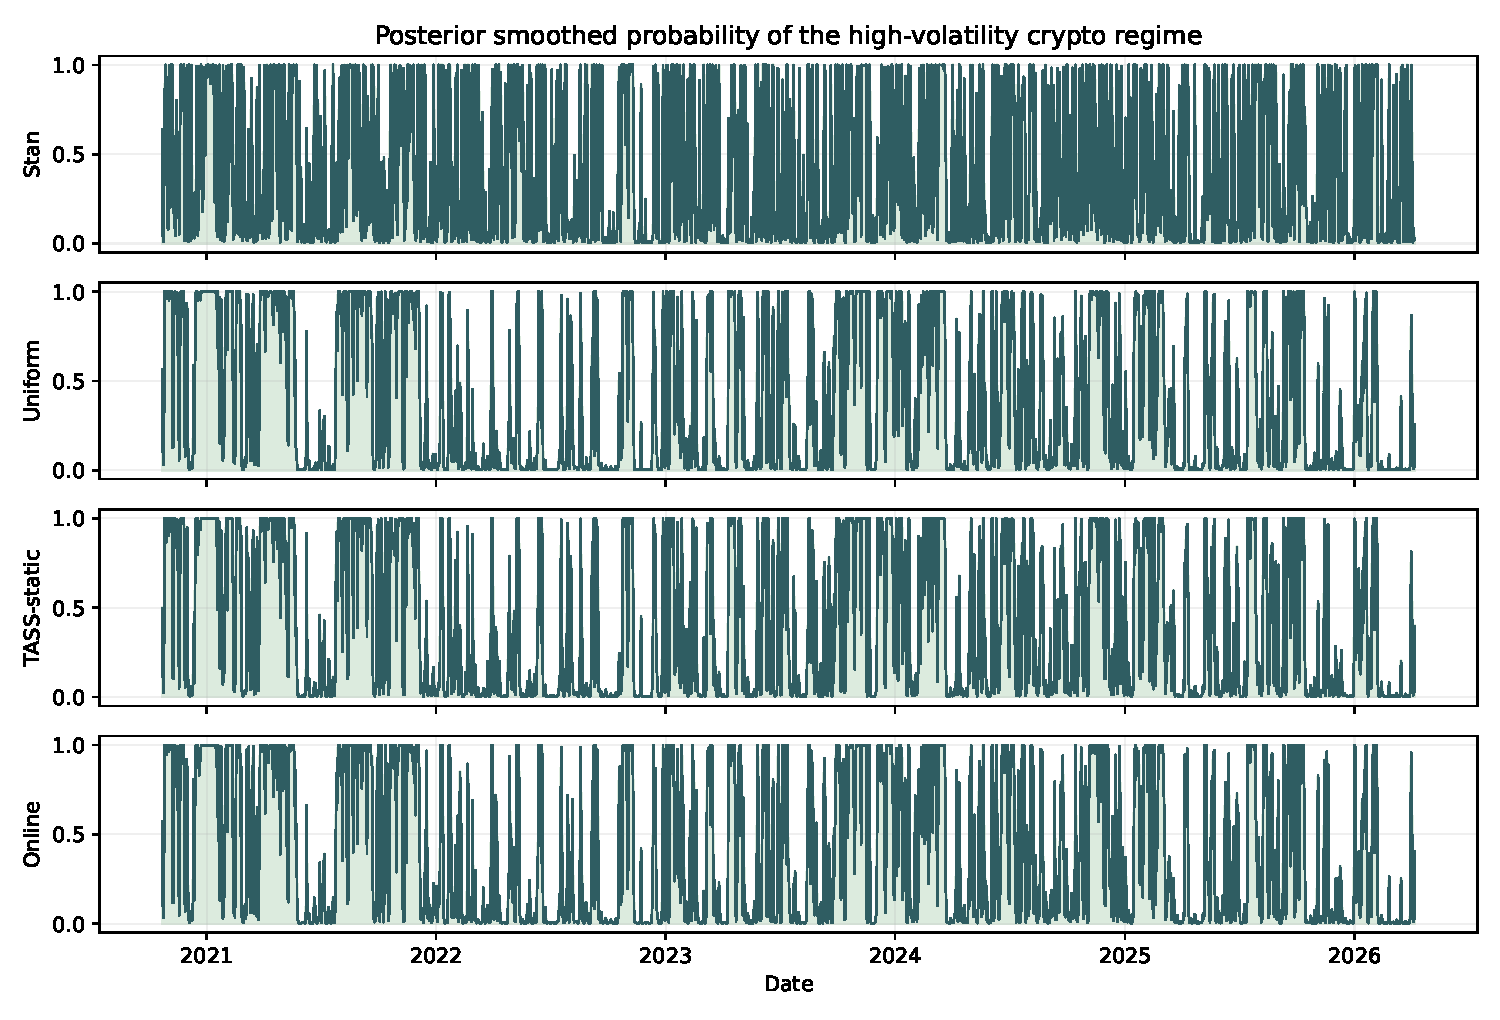
\includegraphics[height=0.78\textheight]{crypto_k2_state_probabilities.pdf}
  \end{center}
\end{frame}

\begin{frame}{The painful diagnostic result}
  \begin{center}
    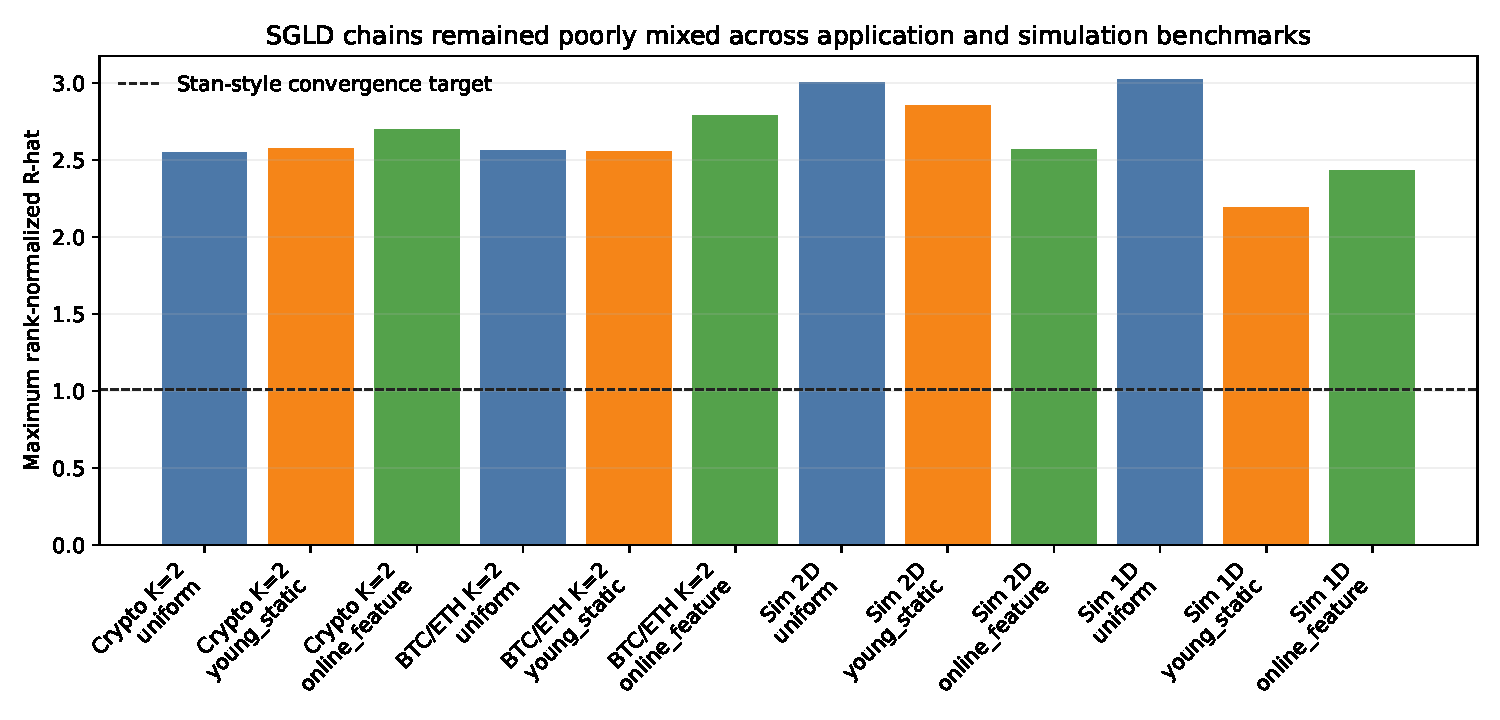
\includegraphics[height=0.58\textheight]{sgmcmc_mixing_summary.pdf}
  \end{center}

  \begin{block}{Interpretation}
    \small
    Good-looking state probabilities are not enough. Cross-chain diagnostics say the SGMCMC posterior samples are not trustworthy yet.
  \end{block}
\end{frame}

\begin{frame}{Why this does not kill the online idea}
  \begin{itemize}
    \item Online weighting is a gradient-estimator variance reduction tool.
    \item Our failures were dominated by HMM posterior geometry:
    \begin{itemize}
      \item label switching,
      \item weakly identified third state,
      \item transition/covariance coupling,
      \item finite-step SGLD bias.
    \end{itemize}
    \item If posterior geometry is the bottleneck, better block weights cannot magically fix the chain.
  \end{itemize}

  \begin{block}{Cleaner claim}
    Online weighting deserves a benchmark where gradient-estimator variance is the bottleneck and feature-gradient relationships evolve over time.
  \end{block}
\end{frame}

\begin{frame}{Takeaways}
  \begin{enumerate}
    \item TASS is principled: sample subsequences in proportion to parameter-specific gradient importance.
    \item Online weighting helps when importance is heterogeneous, feature-predictable, and nonstationary.
    \item The actual crypto stress task matches that regime; online is the best risk forecaster.
    \item $K=2$ rolling-standardized Gaussian HMM is the defensible Bayesian regime model.
    \item The SGMCMC chains did not mix well enough for posterior claims.
  \end{enumerate}

  \vspace{0.8em}
  \centering
  \Large
  The mooolah is not in forcing SGLD to work everywhere.\\
  It is in using adaptivity where the math says it should pay.
\end{frame}

\begin{frame}{References}
  \footnotesize
  Ou, R., Young, A. L., Sen, D., and Dunson, D. B. (2024).
  \textit{Targeted Stochastic Gradient MCMC for HMMs with Rare Latent States}.
  Bayesian Analysis.

  \vspace{0.8em}
  Welling, M. and Teh, Y. W. (2011).
  \textit{Bayesian Learning via Stochastic Gradient Langevin Dynamics}.
  ICML.

  \vspace{0.8em}
  Vehtari, A., Gelman, A., Simpson, D., Carpenter, B., and Bürkner, P.-C. (2021).
  \textit{Rank-normalization, folding, and localization: An improved R-hat for assessing convergence of MCMC}.
  Bayesian Analysis.
\end{frame}

\end{document}
